\subsection{Label Yield and Reliability Analysis}
\label{sec:results_sop_alignment}

Applying this SOP to a large-scale corpus of $\sim$60K candidate pairs yields compelling insights into LMM evaluation behavior. Crucially, the two models achieve a robust \emph{Preference Agreement} of $95.1\%$ ($56,909 / 59,852$ valid overlapping tasks). Looking at the fundamental sub-scores (Figure~\ref{fig:agreement_analysis}a), the models exhibit high consensus on \emph{Existence} ($89.1\%$) and substantial agreement on \emph{Interaction} ($71.9\%$) and \emph{Appearance} ($69.0\%$). This overwhelmingly high preference consensus demonstrates that the SOP effectively anchors the models' global decision-making, confirming that the intersection-filtered labels are highly reliable and well-suited for training our lightweight evaluator. 

\begin{figure}[t]
    \centering
    \begin{subfigure}[b]{0.32\textwidth}
        
\includegraphics[width=\textwidth]{figures/overall_agreement.pdf}
        \caption{By Evaluation Dimension}
        \label{fig:agree_dim}
    \end{subfigure}
    \hfill
    \begin{subfigure}[b]{0.32\textwidth}
        
\includegraphics[width=\textwidth]{figures/agreement_by_subject.pdf}
        \caption{By Subject Count}
        \label{fig:agree_subj}
    \end{subfigure}
    \hfill
    \begin{subfigure}[b]{0.32\textwidth}
        
\includegraphics[width=\textwidth]{figures/agreement_by_tag.pdf}
        \caption{By Spatial Relationship}
        \label{fig:agree_tag}
    \end{subfigure}
    \caption{Cross-model agreement analysis on $\sim$60K tasks between \texttt{gemini-2.5-flash} and \texttt{gemini-3.1-flash-lite-preview}. (a) Models reliably converge on global preference but exhibit higher variance on fine-grained appearance. (b) Counter-intuitively, preference agreement increases with the number of subjects, as catastrophic compositional failures in dense scenes make the ``less collapsed'' image trivially obvious. (c) Explicitly prompted interactions provide stronger contextual grounding, yielding the highest agreement.}
    \label{fig:agreement_analysis}
\end{figure}

Furthermore, analyzing the preference agreement by scene complexity reveals a counter-intuitive trend: agreement \emph{increases} with the number of subjects (Figure~\ref{fig:agreement_analysis}b). The preference consensus is $91.1\%$ for 2-subject prompts, but rises steadily to $93.4\%$ (4 subjects), $97.7\%$ (6 subjects), and $98.1\%$ (8 subjects). We hypothesize this is because dense multi-subject generation remains exceedingly difficult for current diffusion models; in 8-subject scenarios, candidate images often suffer from catastrophic compositional failures, making the choice between a partially successful image and a completely collapsed image trivially obvious to both judges. Finally, analyzing by spatial relationship (Figure~\ref{fig:agreement_analysis}c) shows that scenes requiring \emph{occlusion with interaction} yield the highest agreement ($97.2\%$), whereas \emph{occlusion without interaction} yields the lowest ($92.8\%$), suggesting that explicitly prompted interactions provide stronger contextual grounding for the LMMs to anchor their judgments.

\paragraph{Qualitative Analysis of SOP Effectiveness.}
To further validate the robustness of our SOP, we qualitatively examine cases where both \texttt{gemini-2.5-flash} and \texttt{gemini-3.1-flash-lite-preview} reach a strict consensus on all sub-scores and the final preference (Figure~\ref{fig:sop_demos}). The externalized \emph{flaw logs} reveal that the LMMs successfully internalize the multi-dimensional constraints defined in the SOP:

\begin{itemize}[leftmargin=*, label=$\bullet$]
    \item \textbf{Action and Target Grounding}: In Figure~\ref{fig:sop_demos}(a), the LMMs correctly penalize Candidate B for hallucinating an interaction target (using a stick instead of hand) and missing a secondary interaction entirely (man not tapping). This demonstrates the SOP's ability to enforce precise semantic adherence.
    \item \textbf{Physical Realism and Spatial Constraints}: Figure~\ref{fig:sop_demos}(b) and (d) highlight strict geometric verification. In (b), the models penalize a mug that is embedded in a strange artifact and floating, violating realistic physics. In (d), both LMMs catch severe scale distortion (an abnormally giant fried chicken), directly applying the ``realistic scale'' constraint mandated by the SOP.
    \item \textbf{Fine-grained Attribute Fidelity}: As seen in Figure~\ref{fig:sop_demos}(c) and (d), the models effectively scrutinize wardrobe and identity details, successfully catching subtle errors such as the wrong donut color (pink instead of chocolate) or an incorrect suitcase color (black instead of white).
    \item \textbf{Robustness in Complex Scenes}: Figure~\ref{fig:sop_demos}(e) demonstrates a 6-subject composition where Candidate B suffers from severe collapse. Despite the density of the scene, both models accurately and consistently isolate multiple concurrent failures across Appearance (wrong clothing) and Interaction (missing petting, closing, and carrying actions).
\end{itemize}

Overall, these qualitative results confirm that the ``errors-first'' scaffolding successfully prevents the LMMs from falling back on holistic aesthetic biases, forcing them to conduct rigorous, localized compositional verification.

\begin{figure}[htbp]
    \centering
    \begin{subfigure}[b]{0.48\textwidth}
        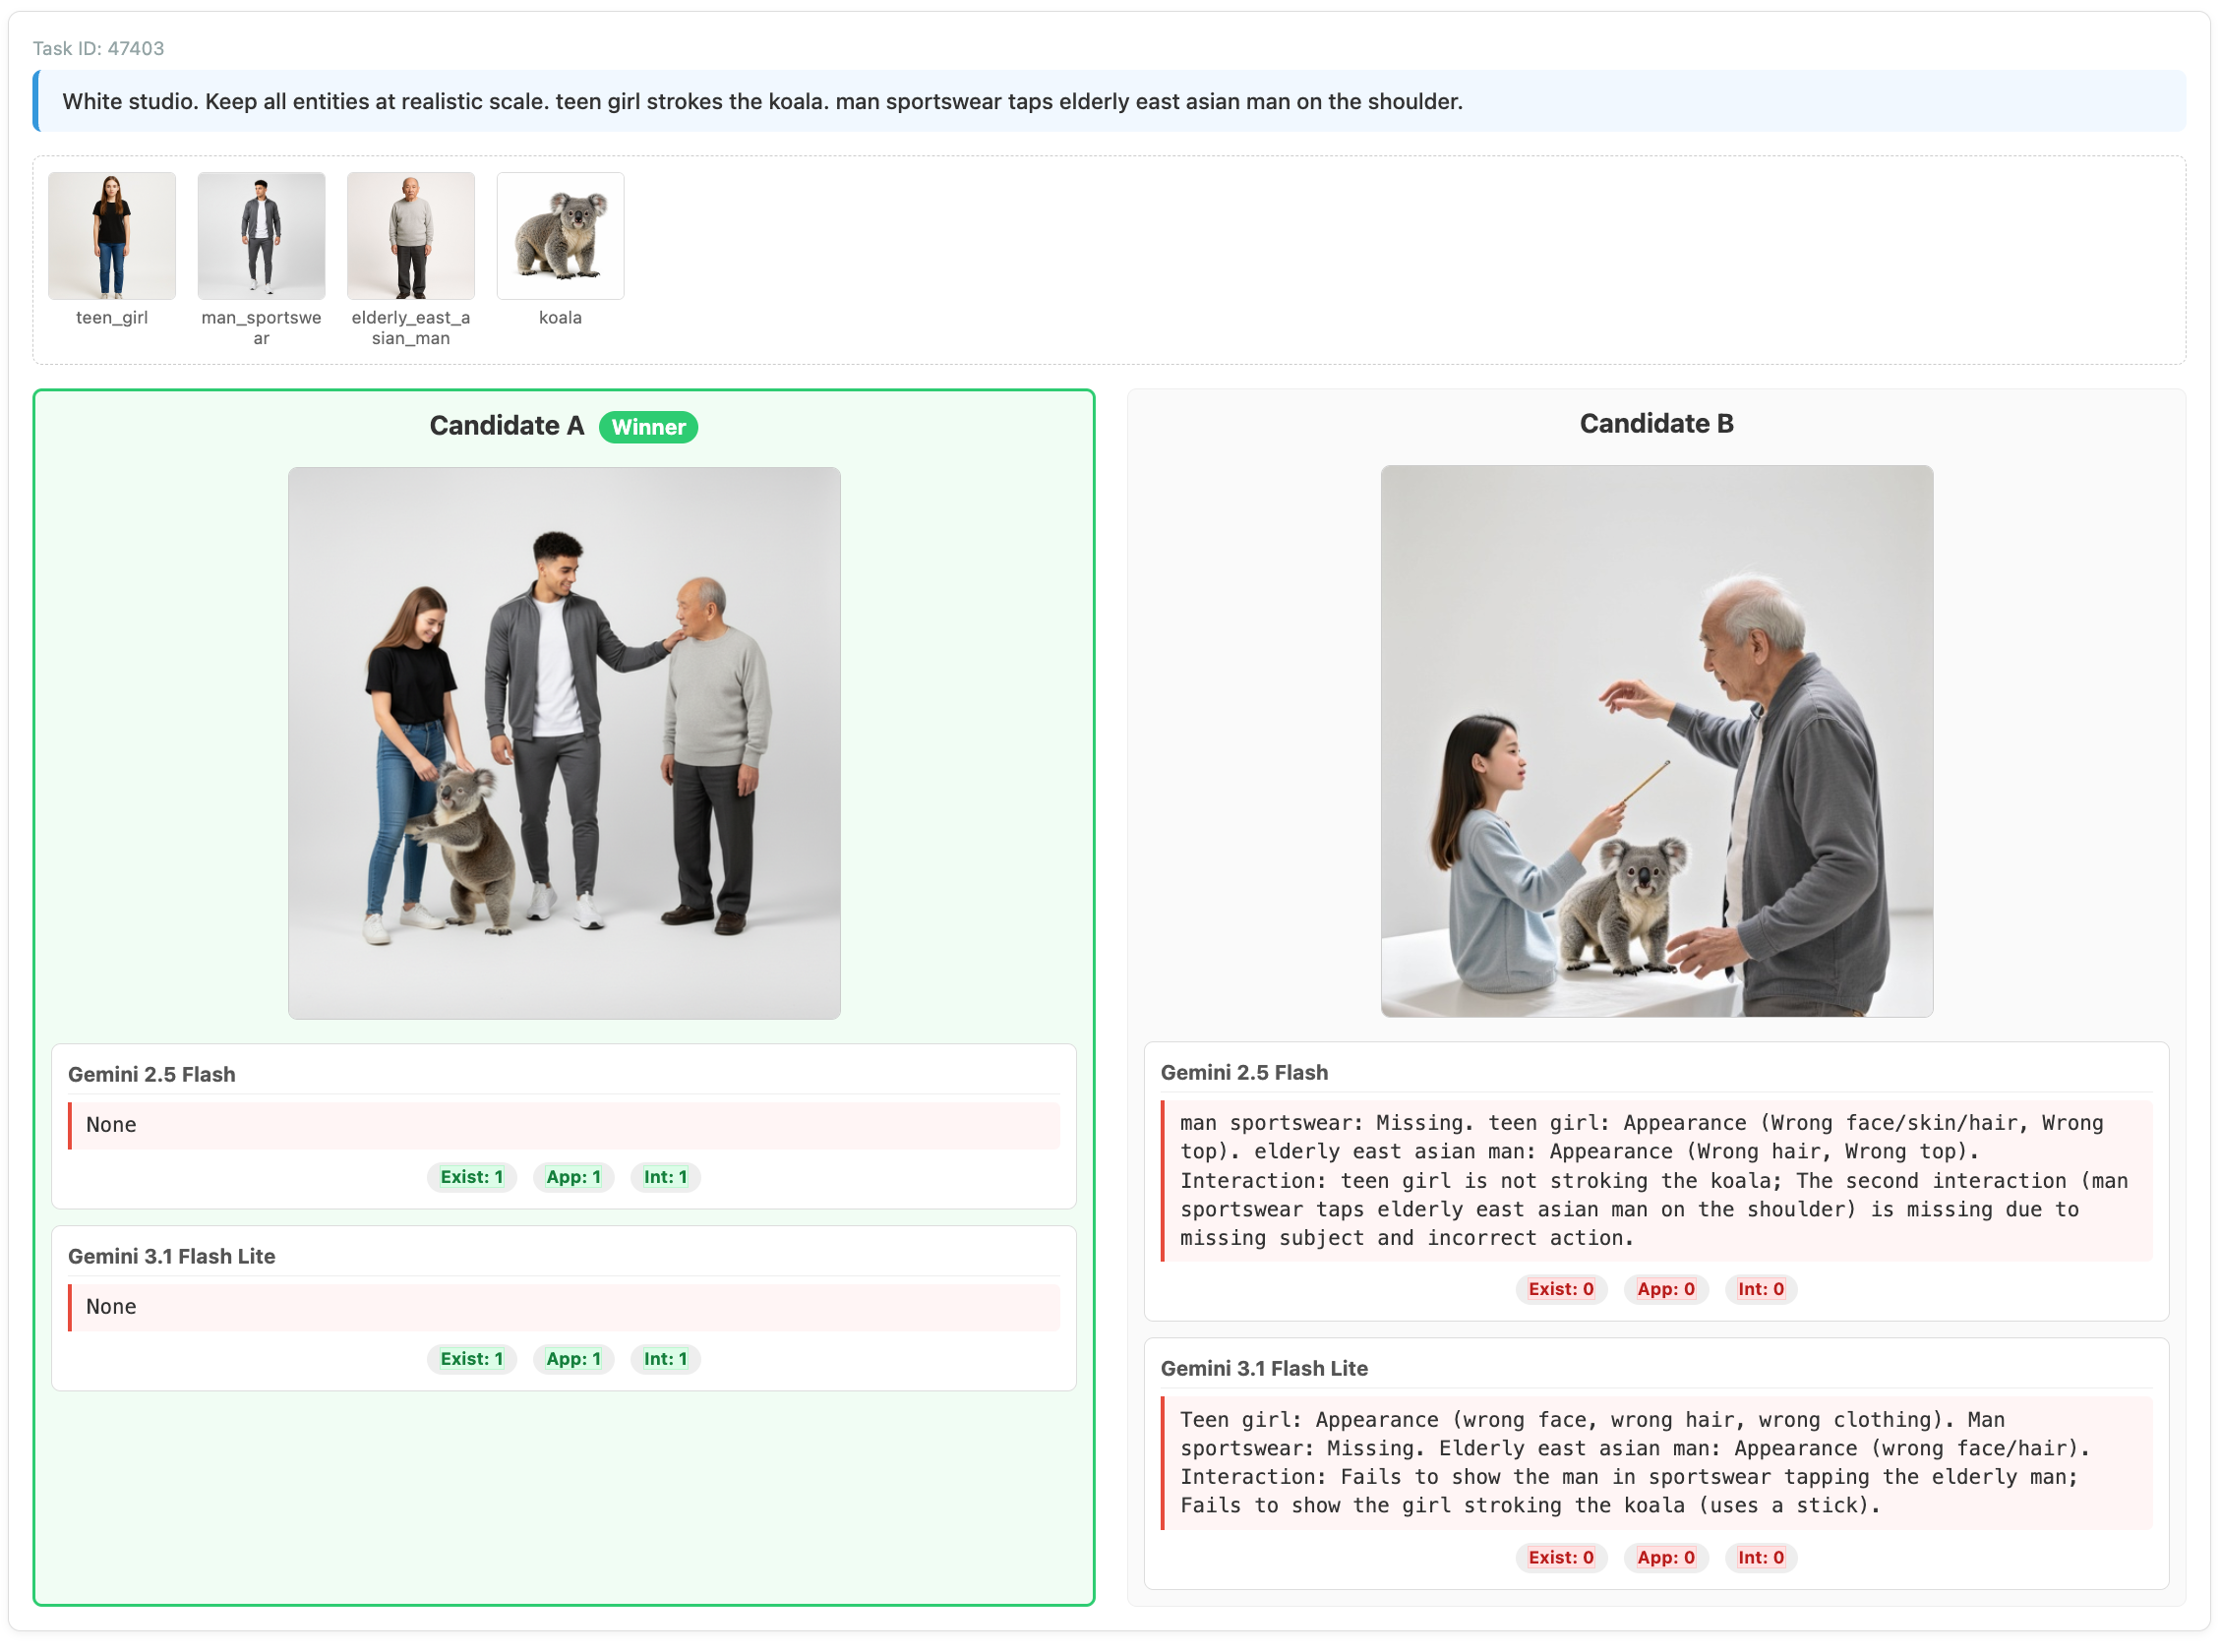
\includegraphics[width=\textwidth]{figures/SOP_demo_1.png}
        \caption{Action and Target Errors}
    \end{subfigure}
    \hfill
    \begin{subfigure}[b]{0.48\textwidth}
        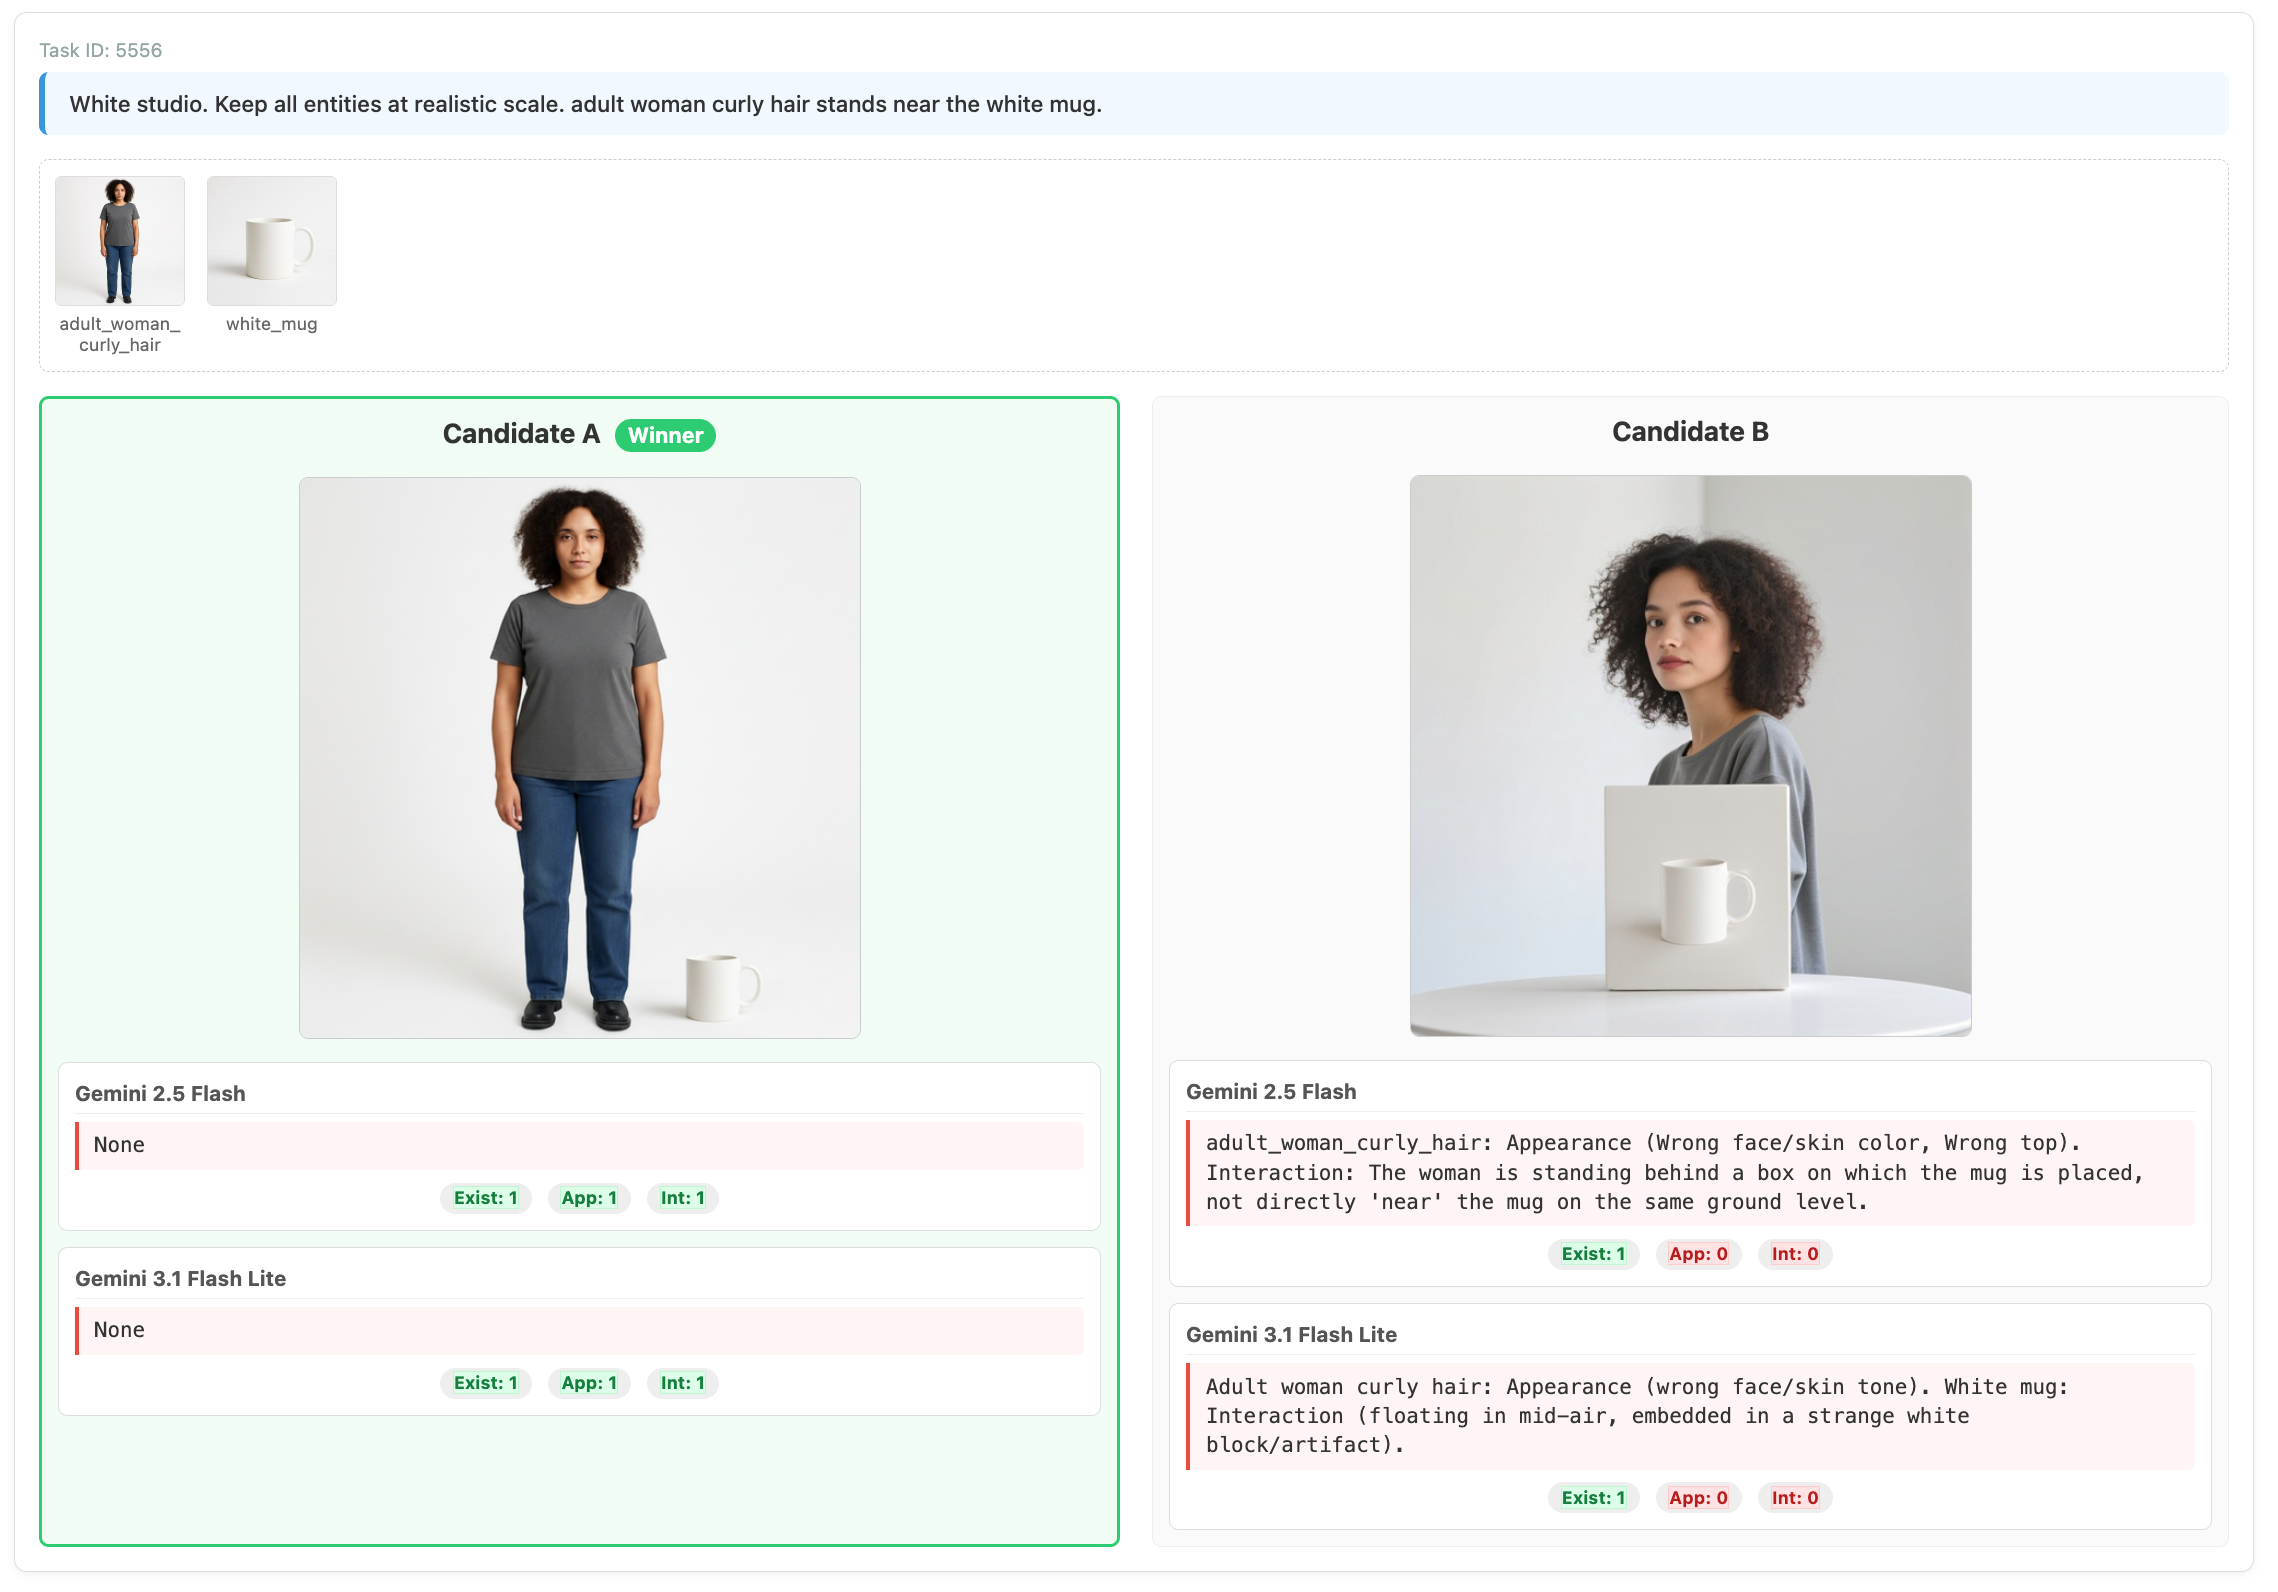
\includegraphics[width=\textwidth]{figures/SOP_demo_2.png}
        \caption{Physics and Spatial Violations}
    \end{subfigure}
    \vspace{1em}
    \begin{subfigure}[b]{0.48\textwidth}
        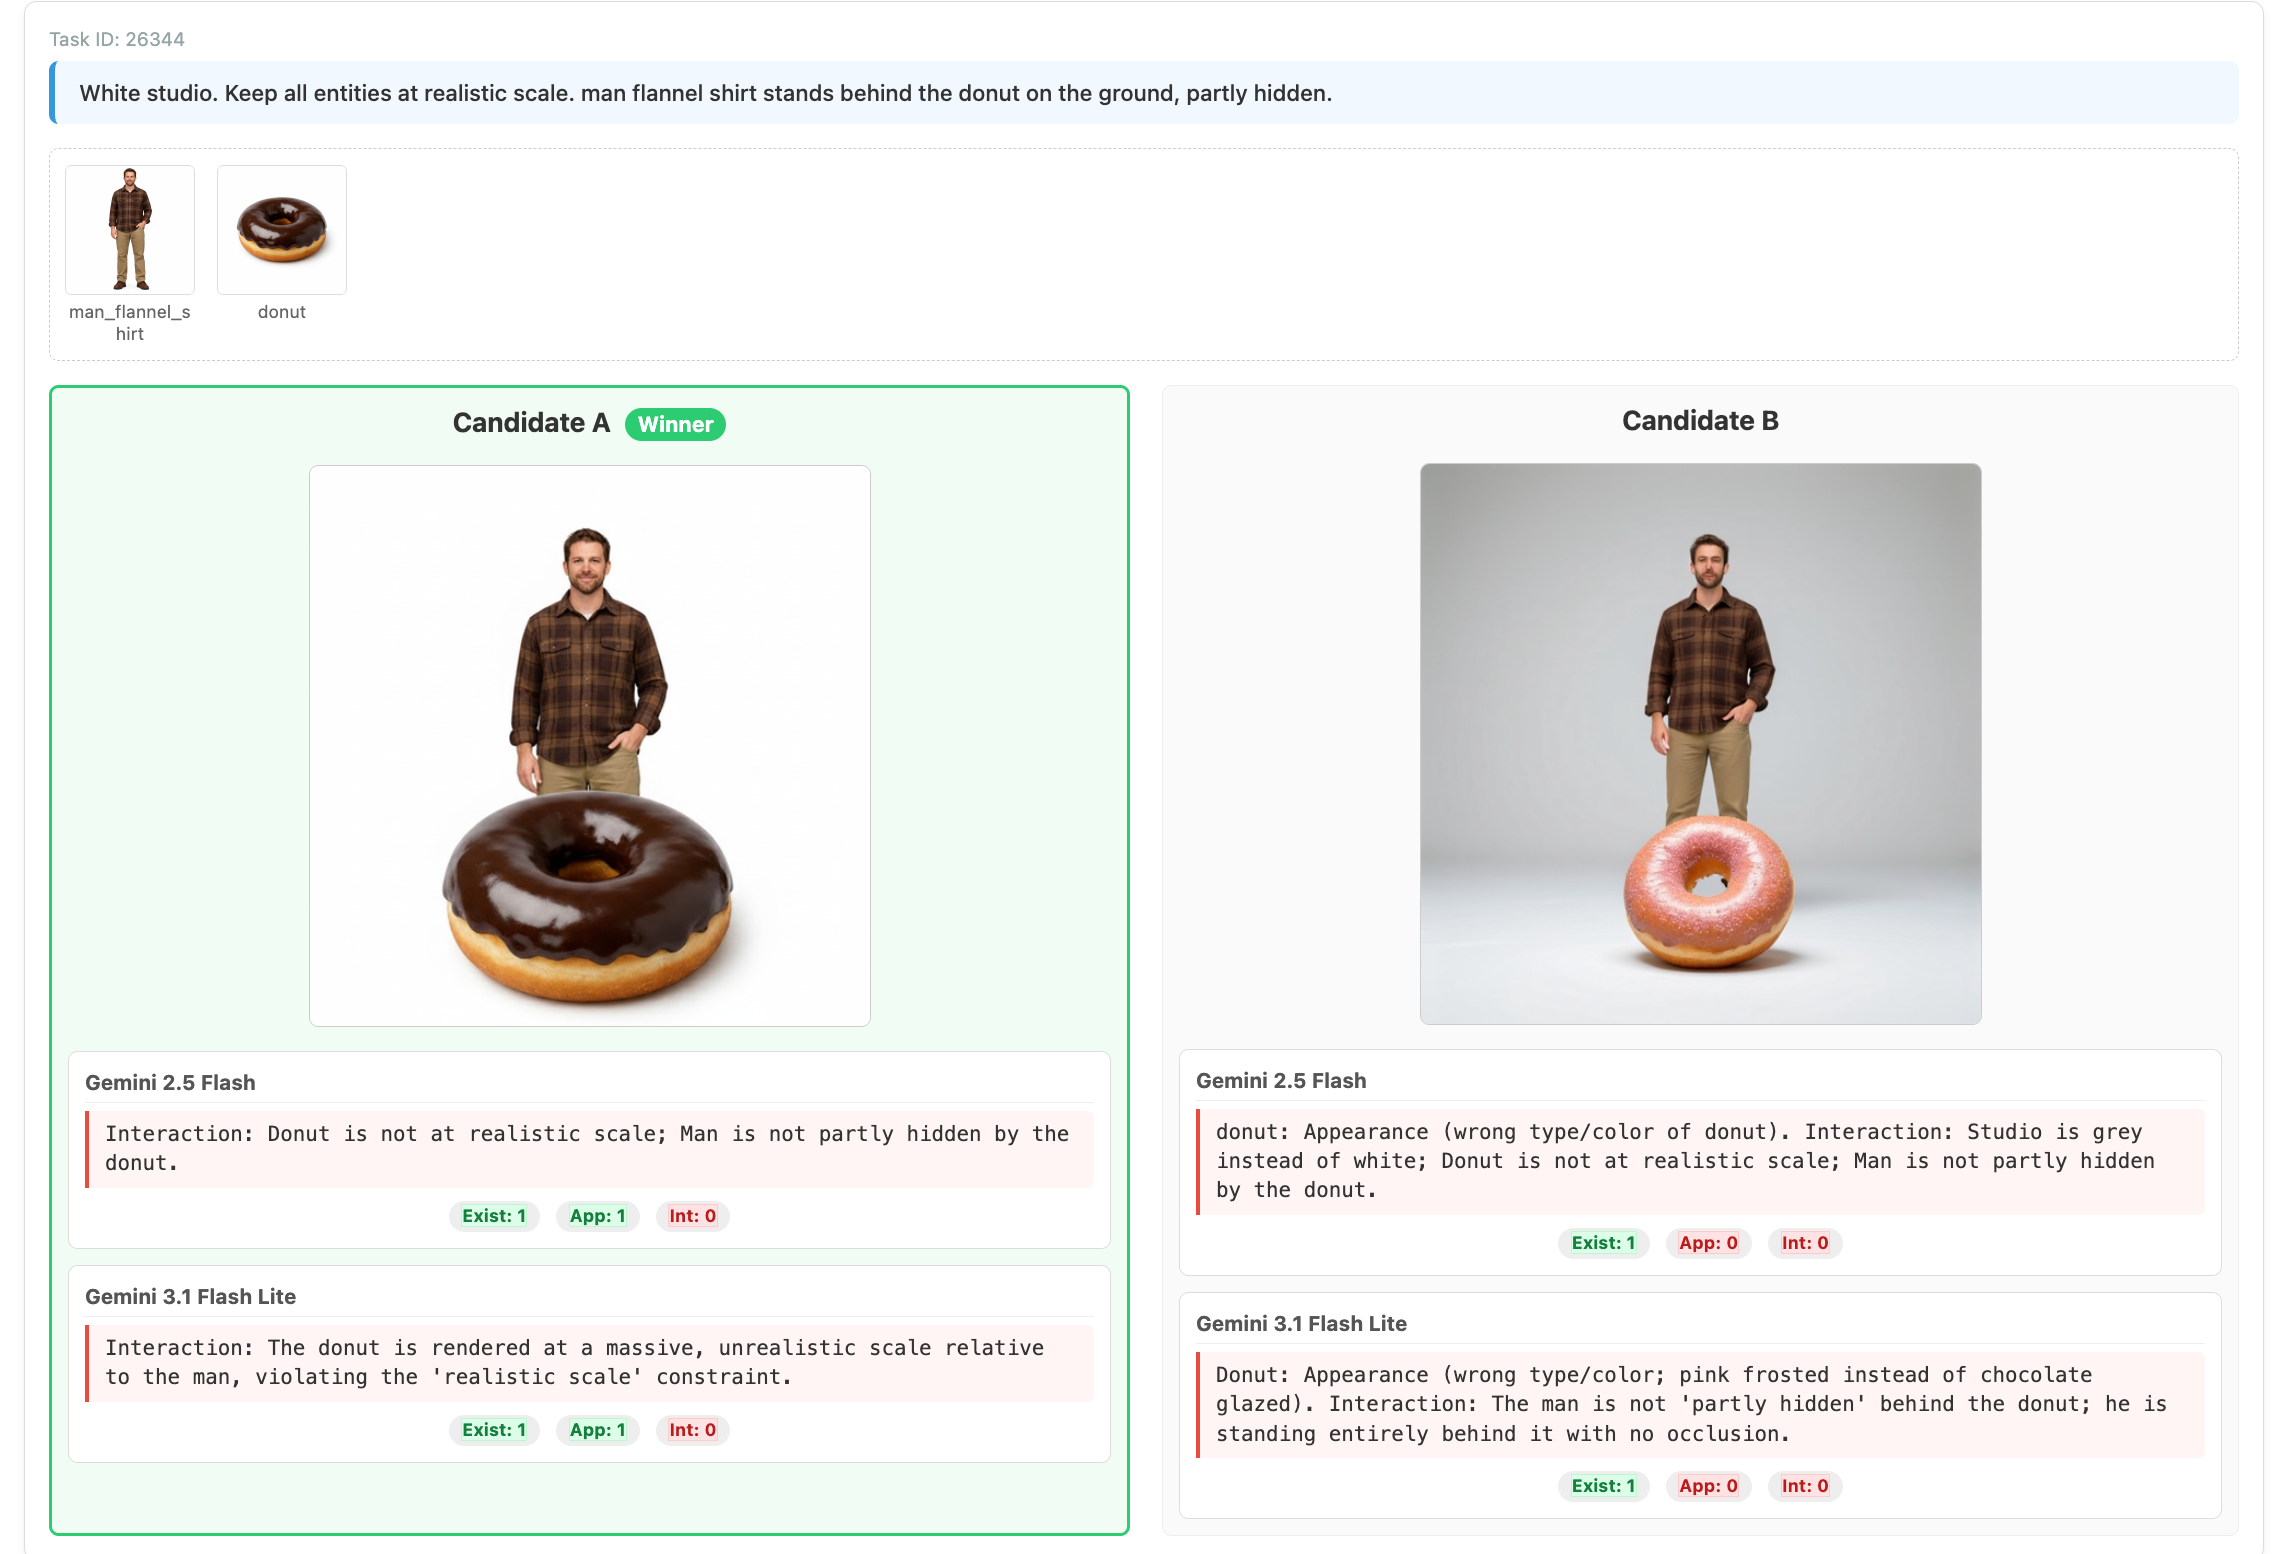
\includegraphics[width=\textwidth]{figures/SOP_demo_3.png}
        \caption{Appearance and Occlusion Errors}
    \end{subfigure}
    \hfill
    \begin{subfigure}[b]{0.48\textwidth}
        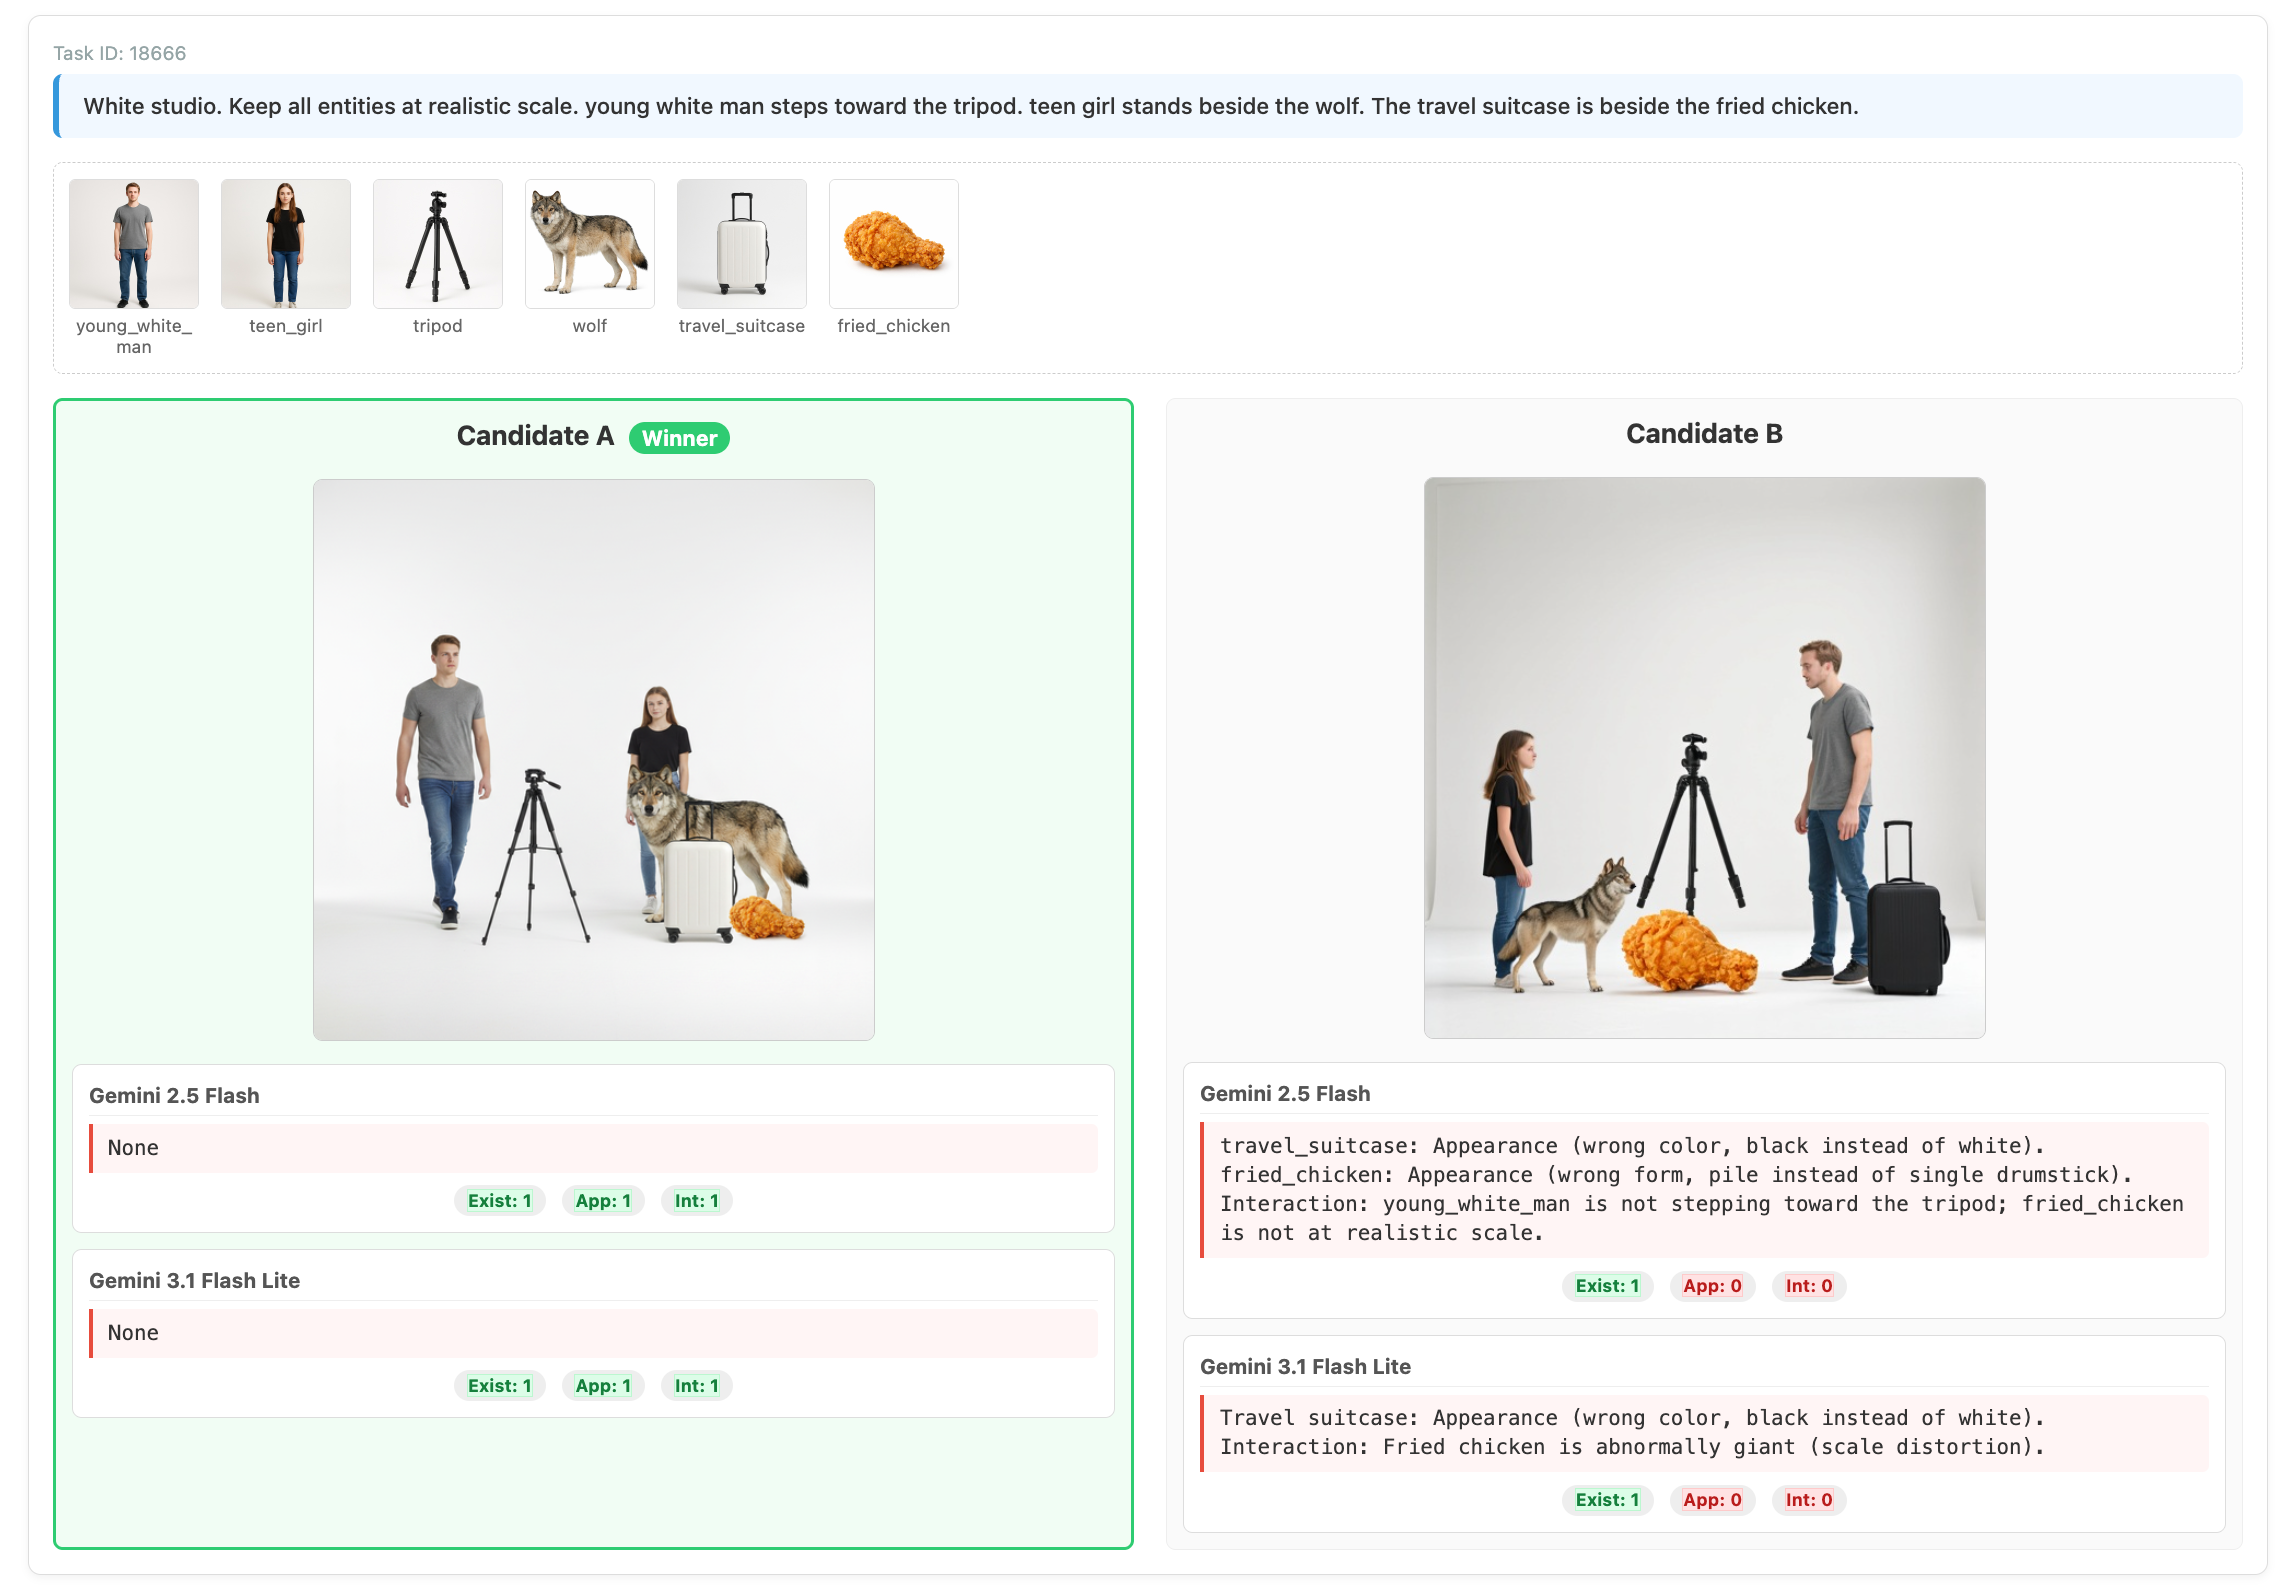
\includegraphics[width=\textwidth]{figures/SOP_demo_4.png}
        \caption{Scale Distortion and Color Mismatch}
    \end{subfigure}
    \vspace{1em}
    \begin{subfigure}[b]{0.8\textwidth}
        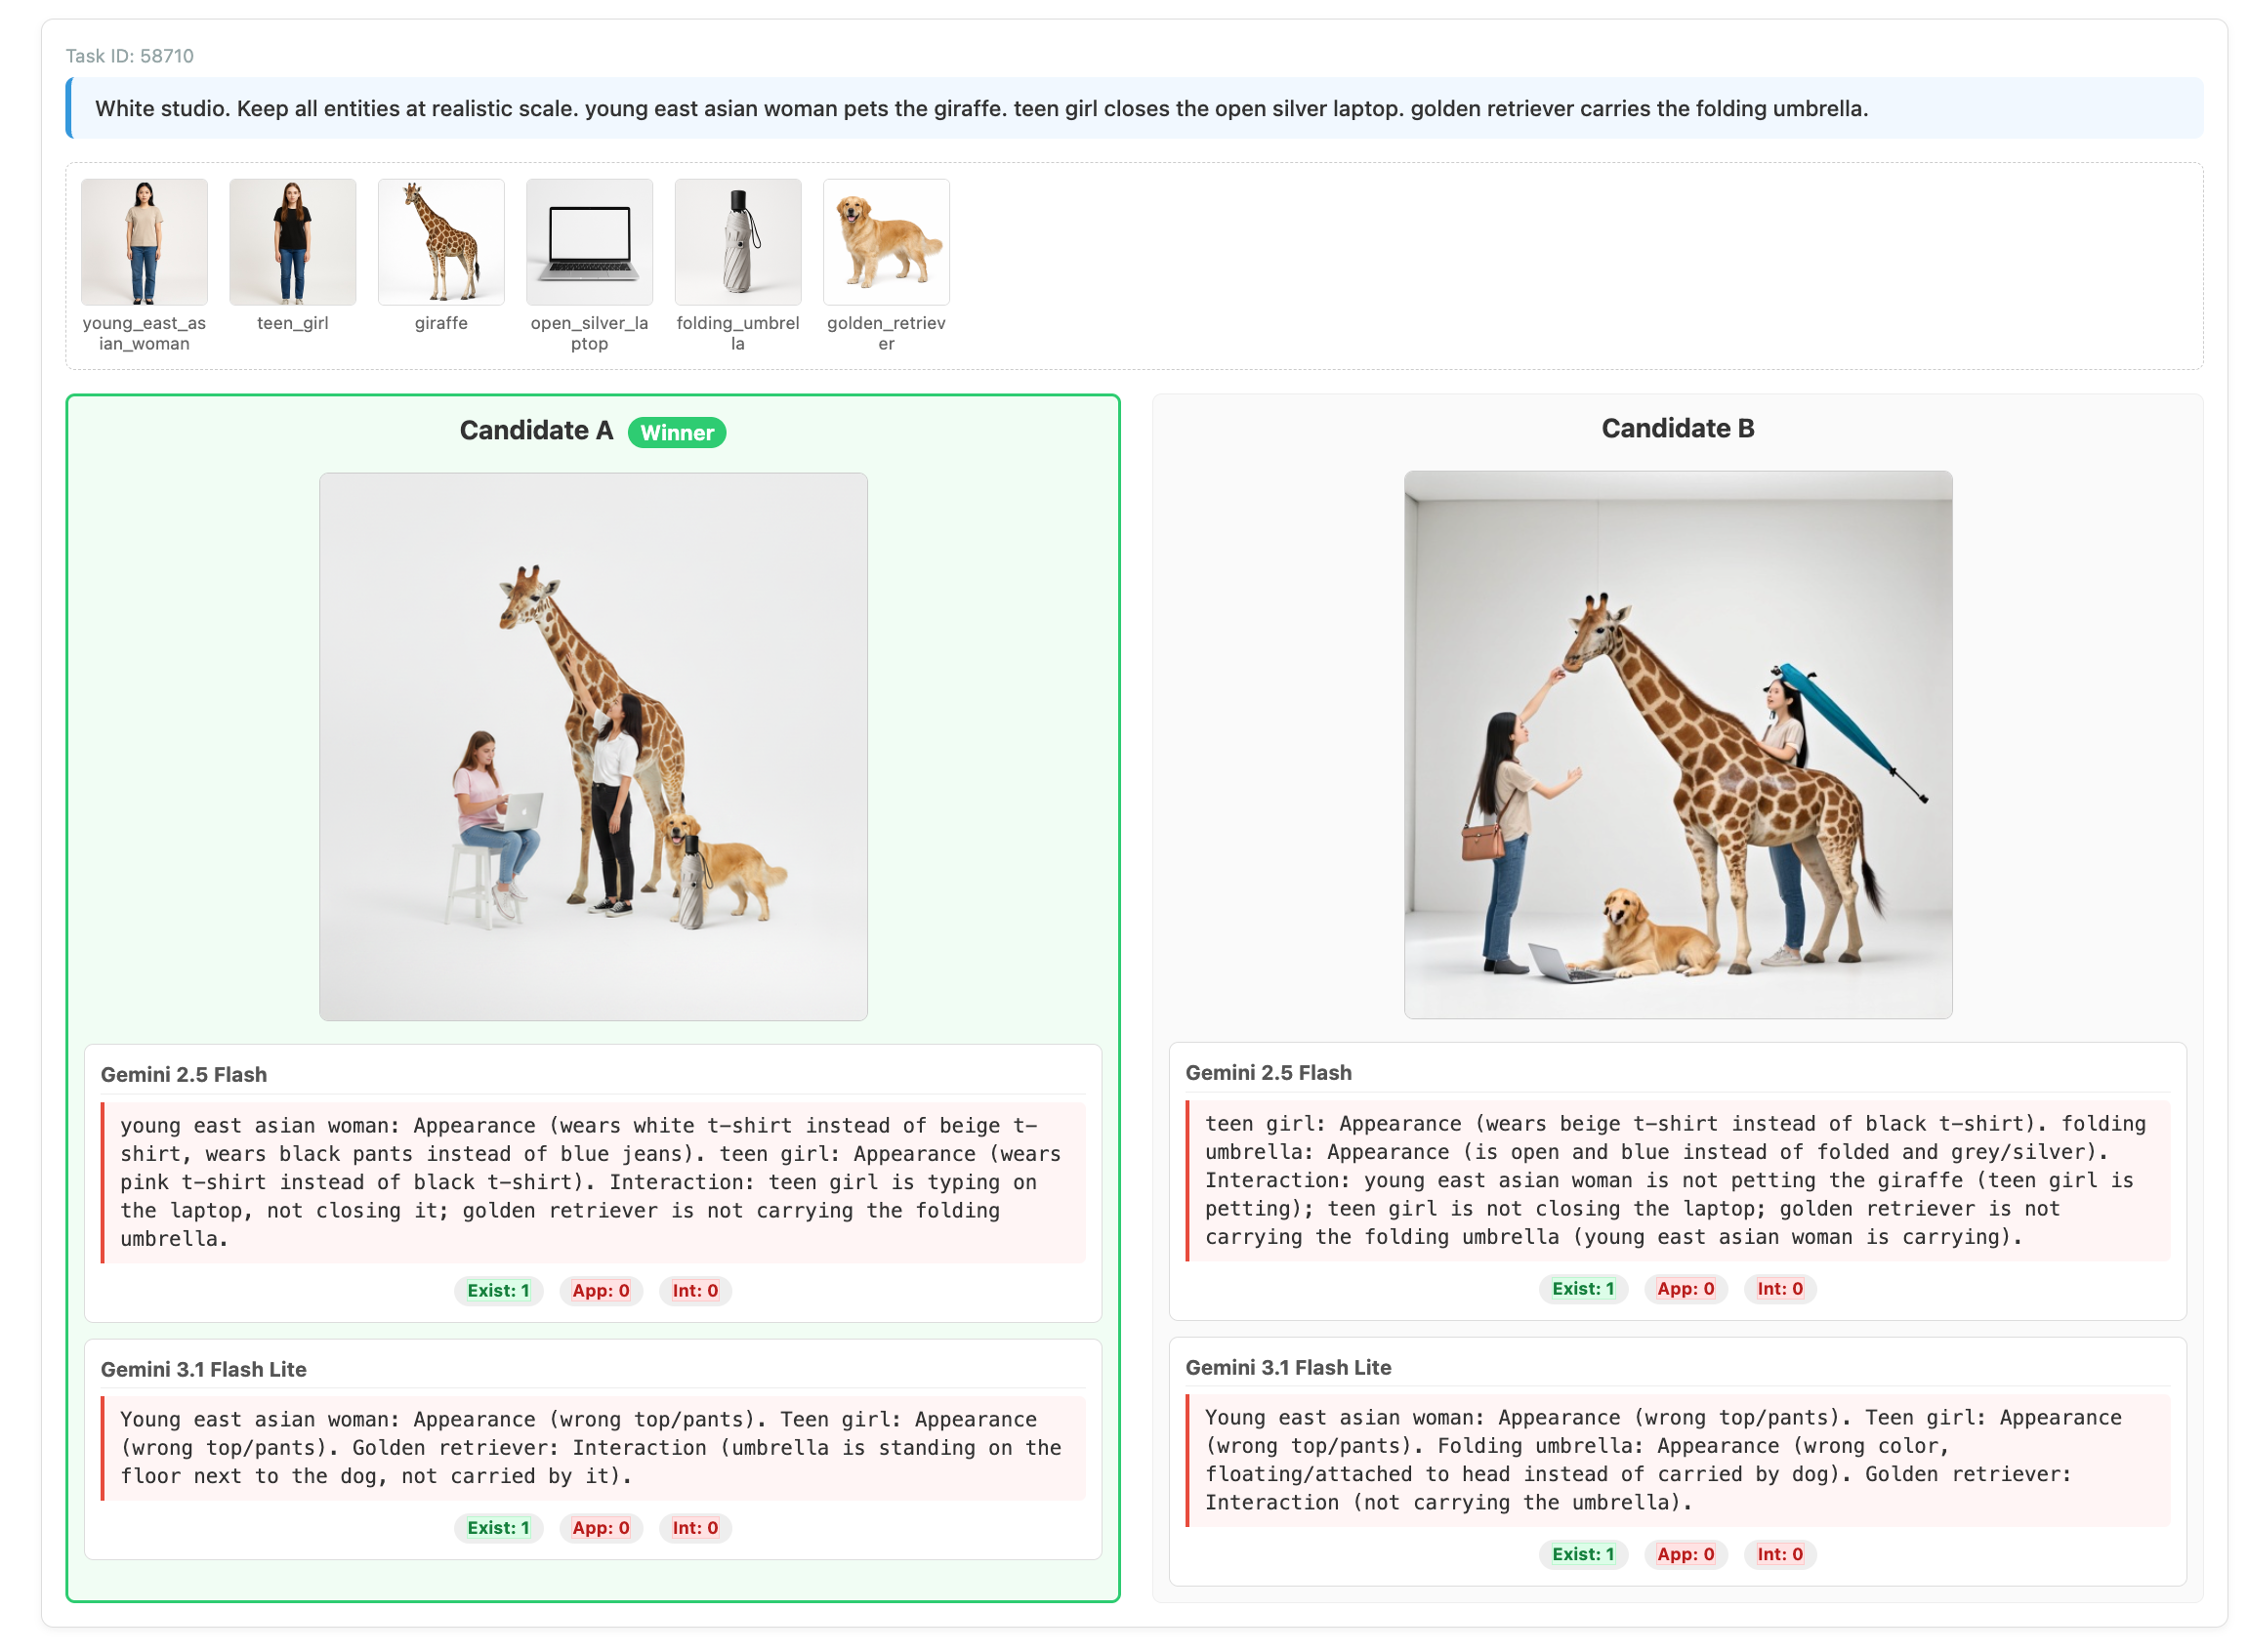
\includegraphics[width=\textwidth]{figures/SOP_demo_5.png}
        \caption{Robust Diagnostics in Highly Complex (6-Subject) Scenes}
    \end{subfigure}
    \caption{Qualitative examples of strict cross-model consensus. The externalized flaw logs demonstrate that both LMMs effectively utilize the SOP to catch fine-grained errors in appearance, physical realism, interaction semantics, and complex multi-subject scaling.}
    \label{fig:sop_demos}
\end{figure}
